\section{Detection Model Results}
\label{sec:ch4_detection_results}

This section summarizes the training behavior and evaluation of the YOLOv8s-seg detection model. We report training/validation loss curves, a confusion matrix, and precision--recall and F1 performance for both bounding boxes and masks.

\subsection{Training and Validation Loss Curves}
Figure~\ref{fig:det_loss_curves_box_seg} presents the training and validation loss curves for the three primary heads in YOLOv8s-seg: bounding-box regression, segmentation, and classification. These curves provide a clear view of convergence behavior and help detect overfitting or underfitting.

After approximately epoch 52, the validation segmentation loss starts to increase relative to the training loss, which indicates the onset of overfitting in the segmentation head. In contrast, both the validation box loss and the validation classification loss become roughly constant after epoch 52, suggesting stable convergence for these two heads.

\begin{figure}[H]
    \centering
    \begin{subfigure}{\textwidth}
        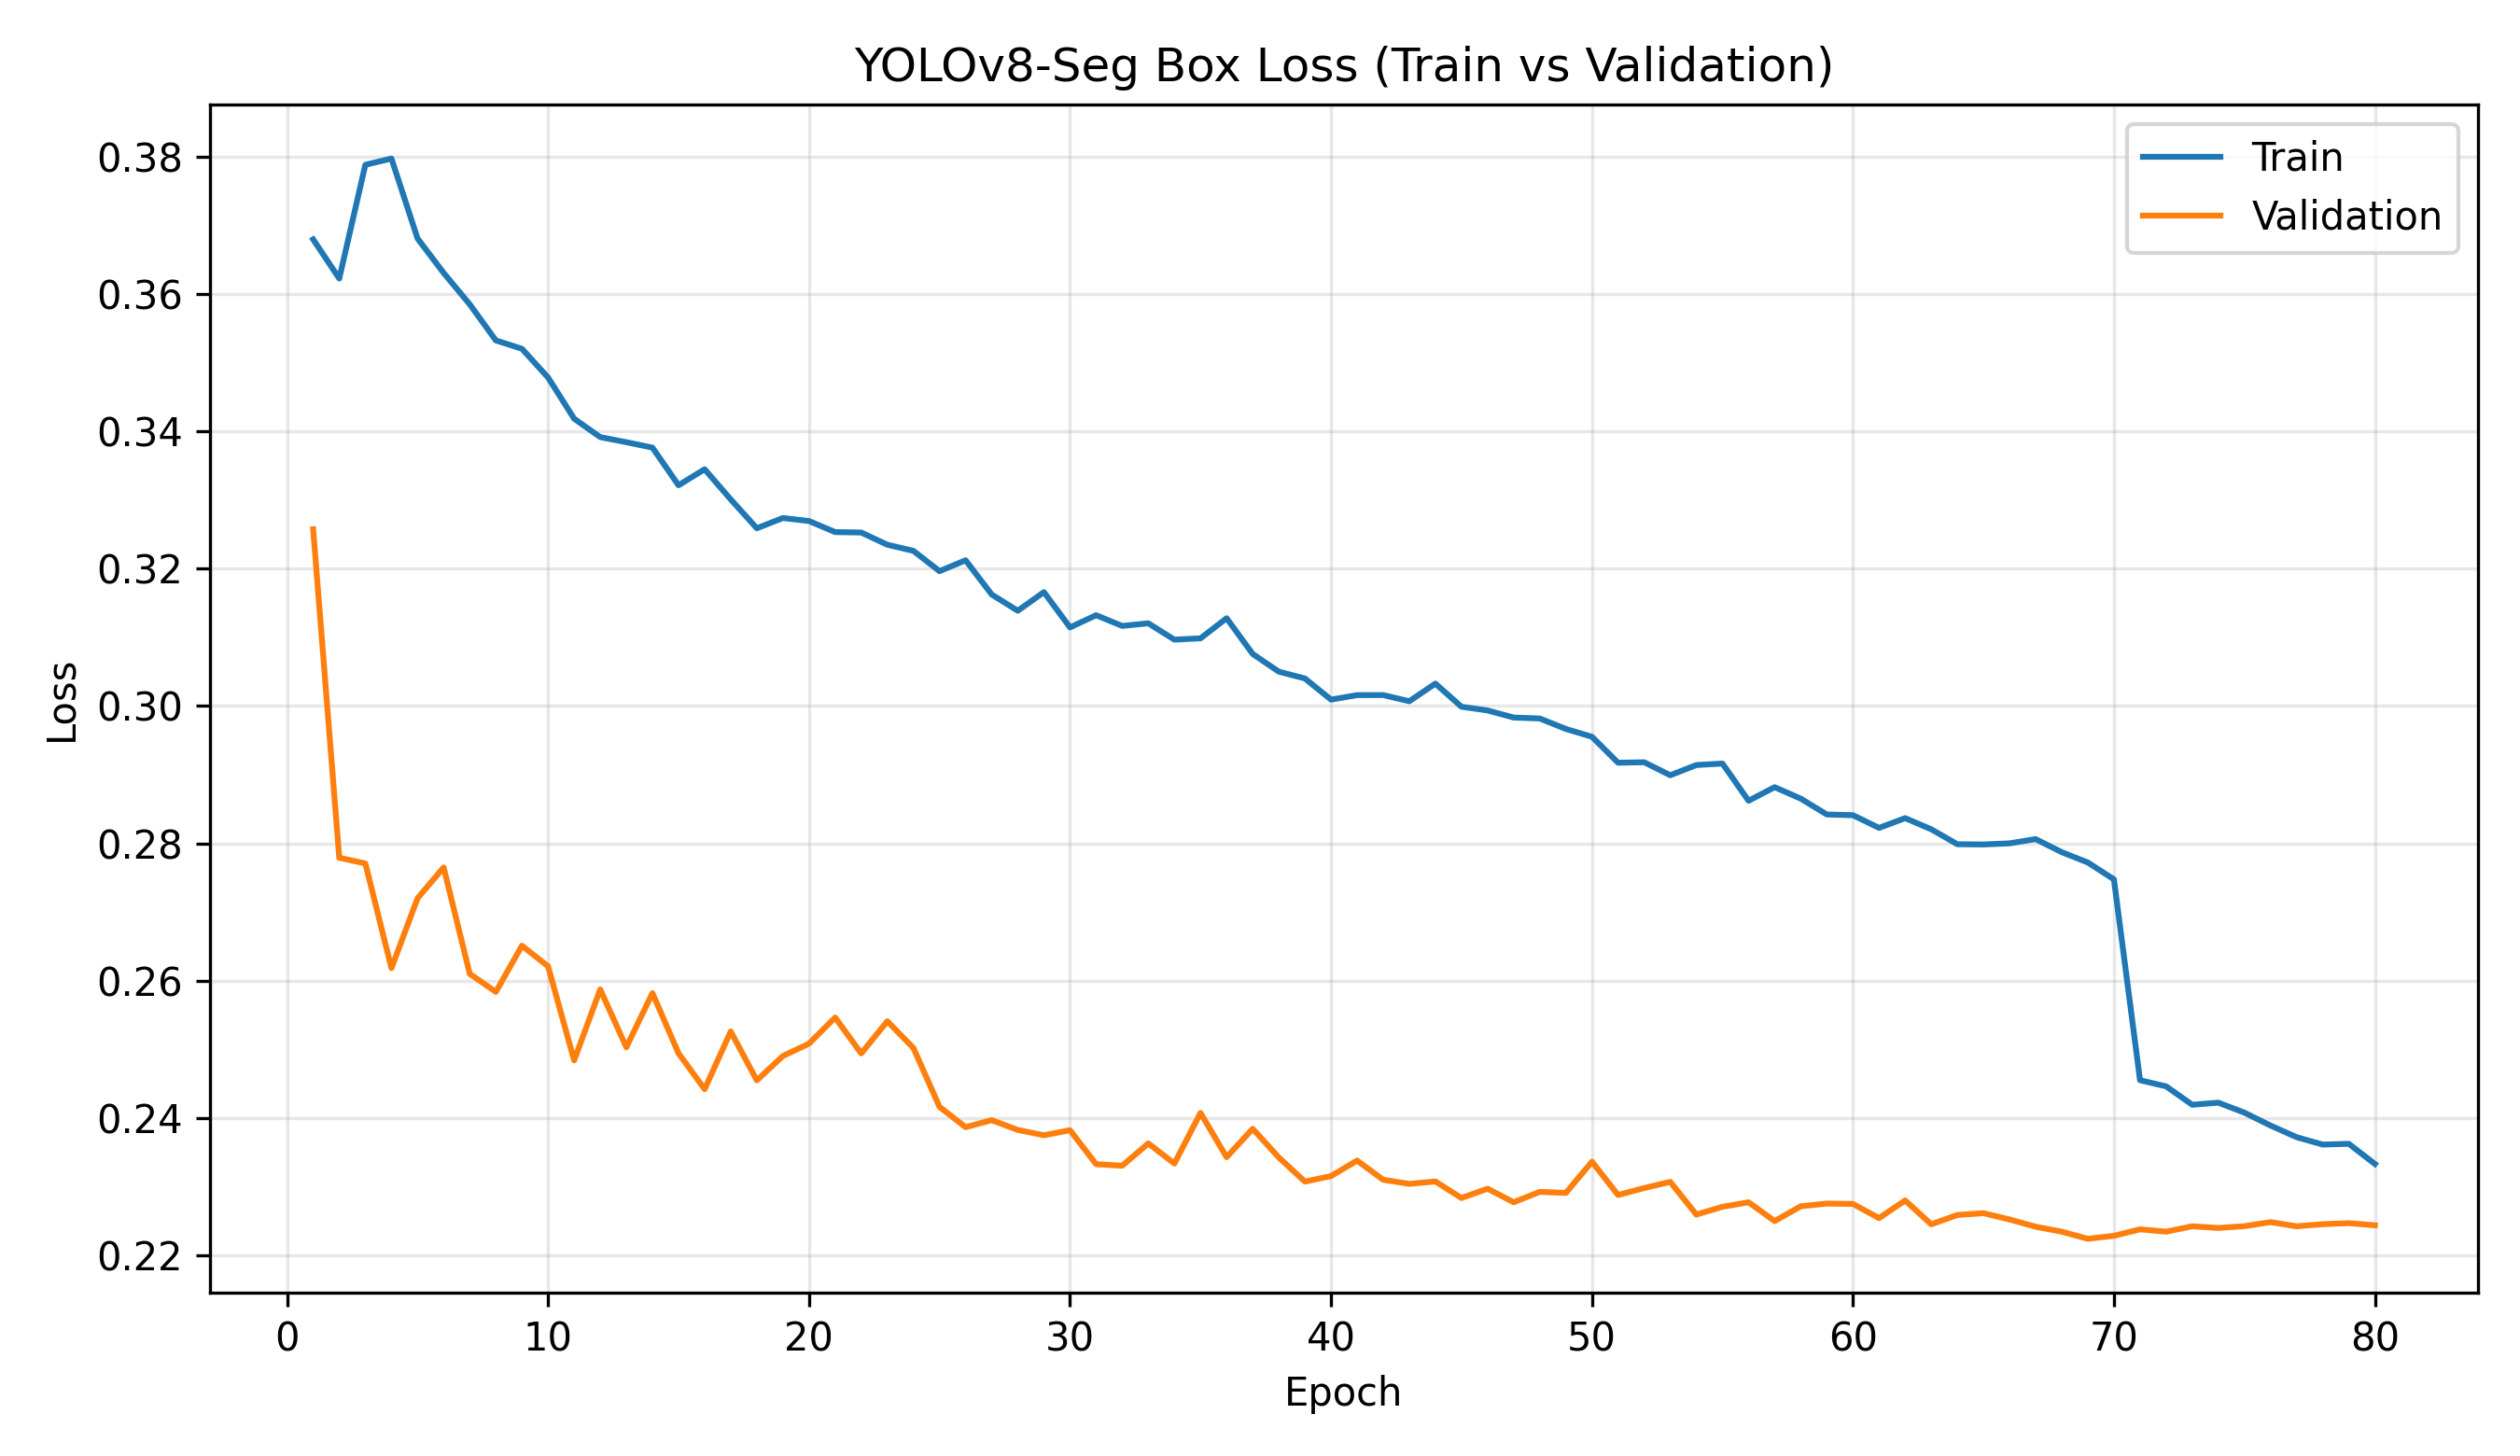
\includegraphics[width=0.92\textwidth]{Figures/chapter4/Detection/curves/thesis_box_loss_train_val.png}
        \caption{Box loss (train vs. val).}
    \end{subfigure}
\end{figure}

\clearpage

\begin{figure}[H]
    \ContinuedFloat
    \centering
    \begin{subfigure}{\textwidth}
        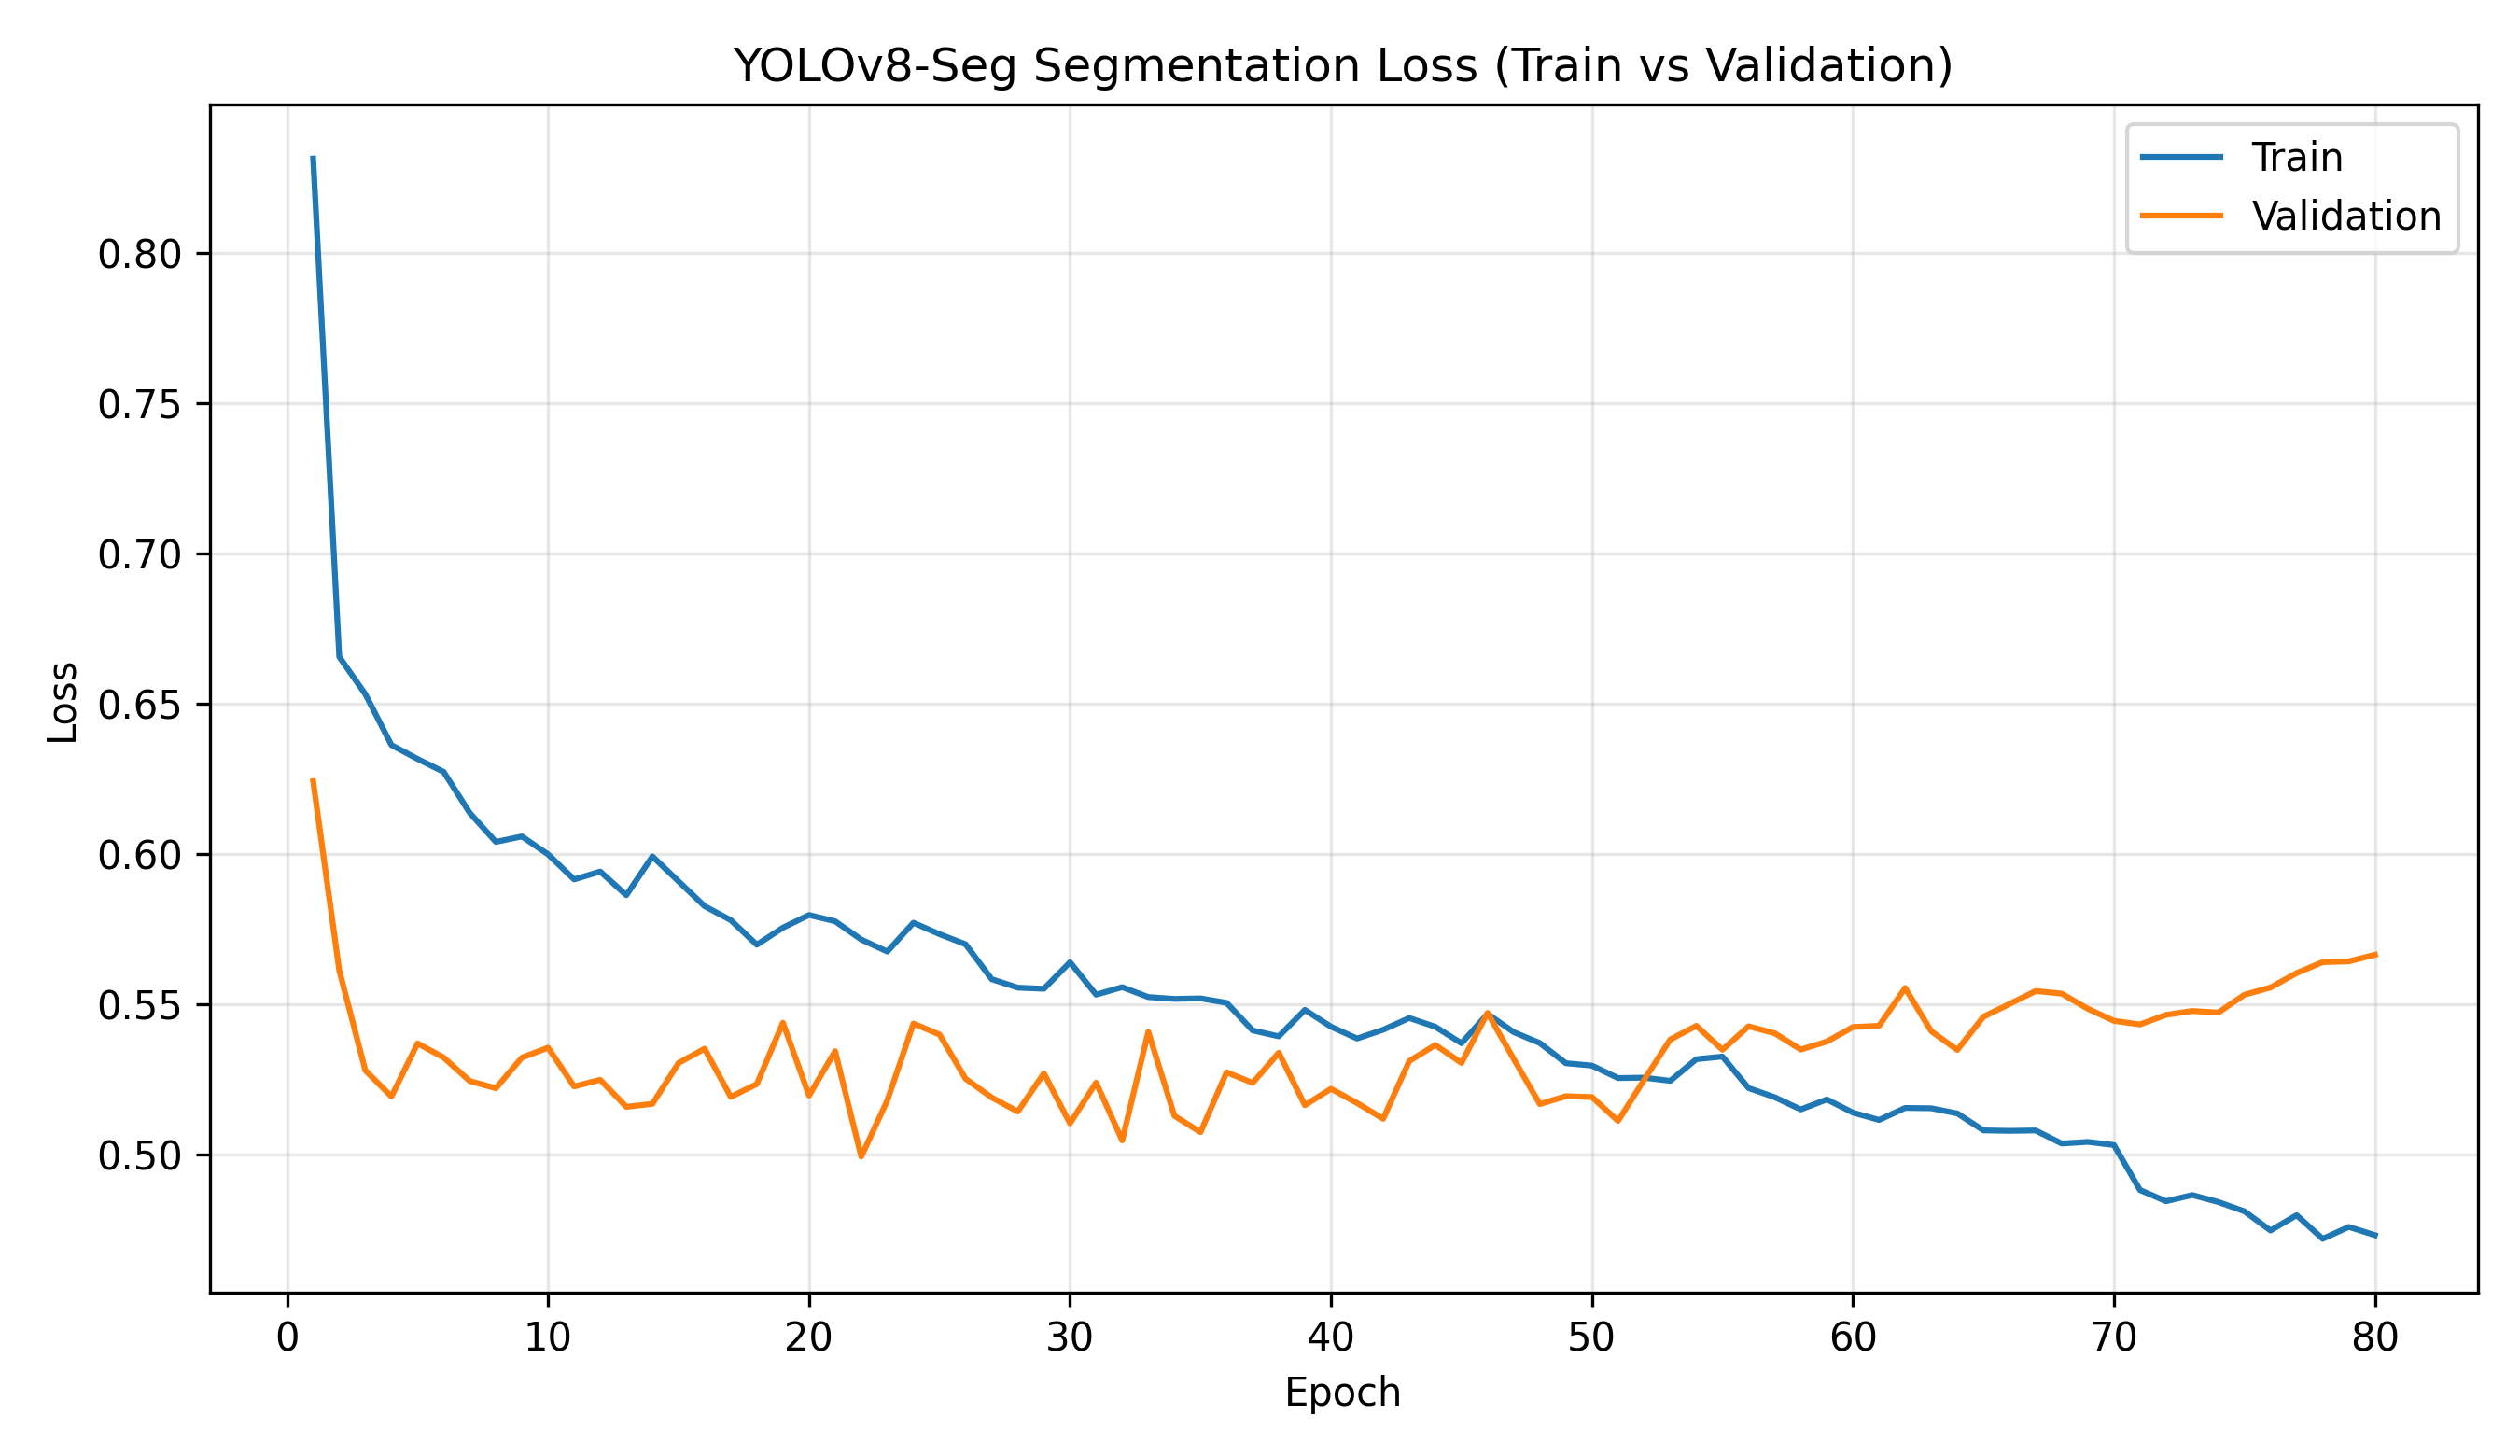
\includegraphics[width=0.95\textwidth]{Figures/chapter4/Detection/curves/thesis_seg_loss_train_val.png}
        \caption{Segmentation loss (train vs. val).}
    \end{subfigure}
    \caption{Training and validation loss curves for box and segmentation heads.}
    \label{fig:det_loss_curves_box_seg}
\end{figure}


\begin{figure}[H]
    \centering
    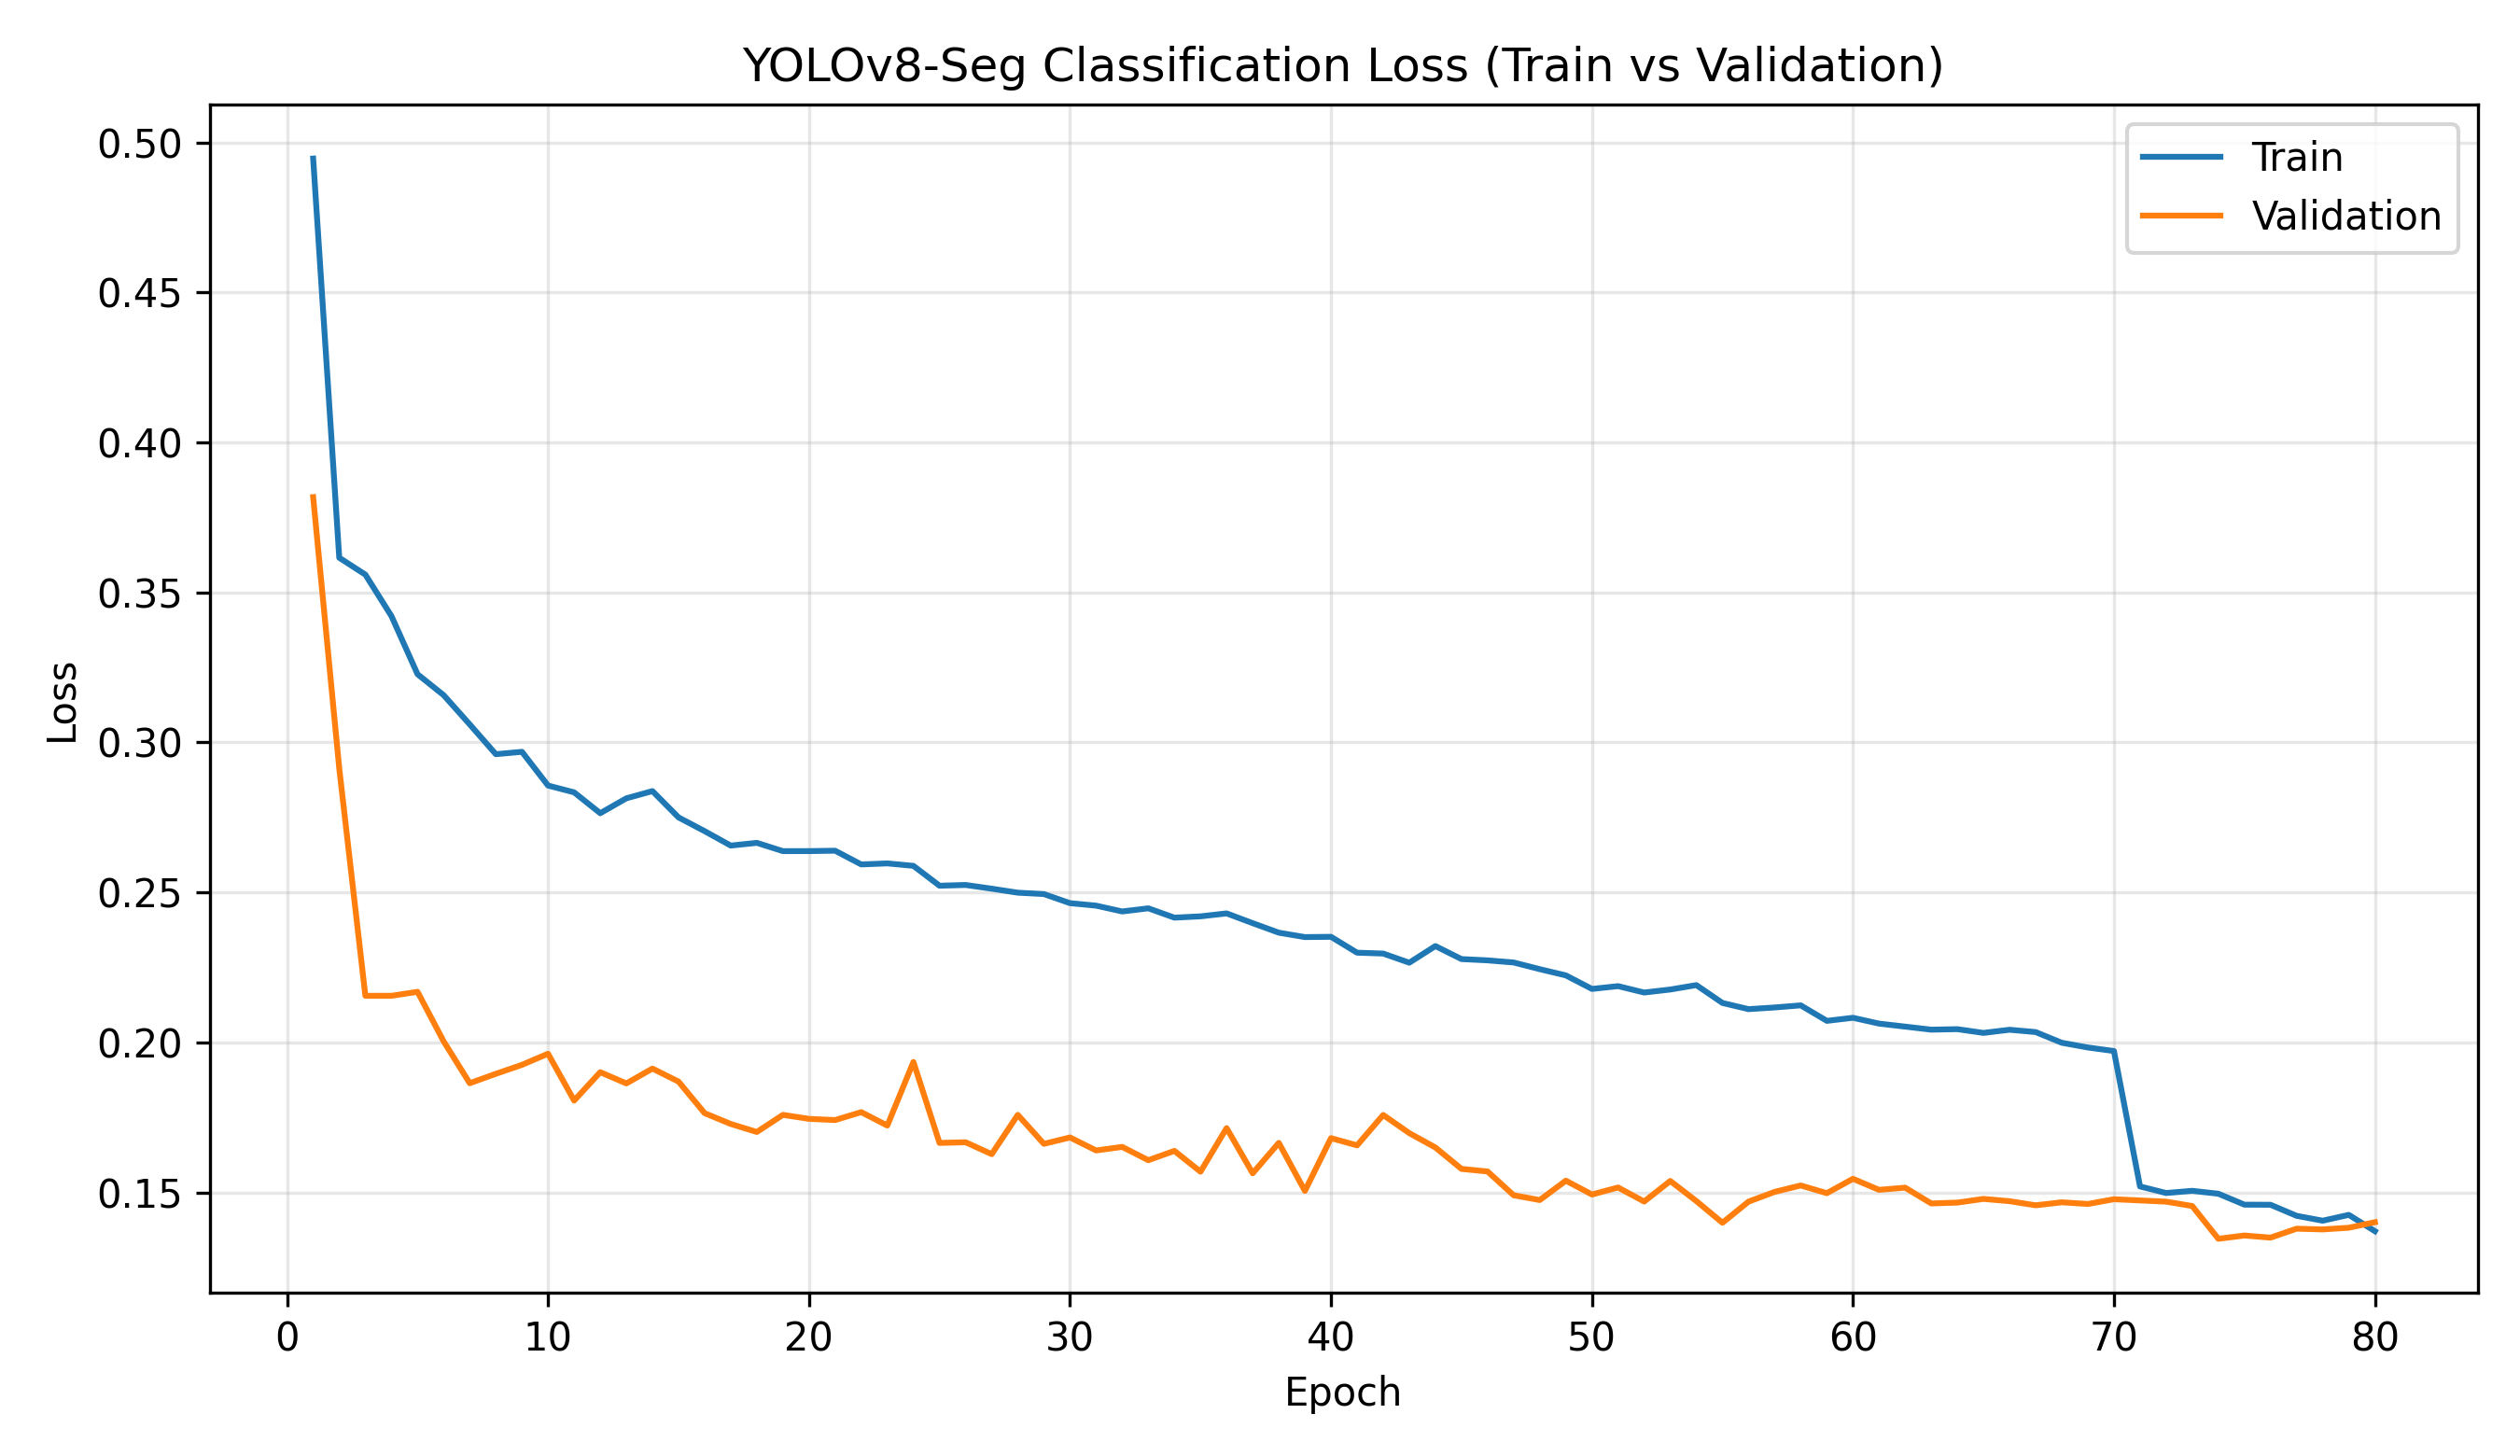
\includegraphics[width=0.95\textwidth]{Figures/chapter4/Detection/curves/thesis_cls_loss_train_val.png}
    \caption{Classification loss (train vs. val).}
    \label{fig:cls_loss_train_val}
\end{figure}

\subsection{Confusion Matrix}
The normalized confusion matrix in Figure~\ref{fig:det_confusion_matrix} summarizes class-level performance. It highlights how frequently each brick class is correctly predicted and where misclassifications occur, which is useful for diagnosing label ambiguity or visually similar shapes.

\begin{figure}[H]
    \centering
    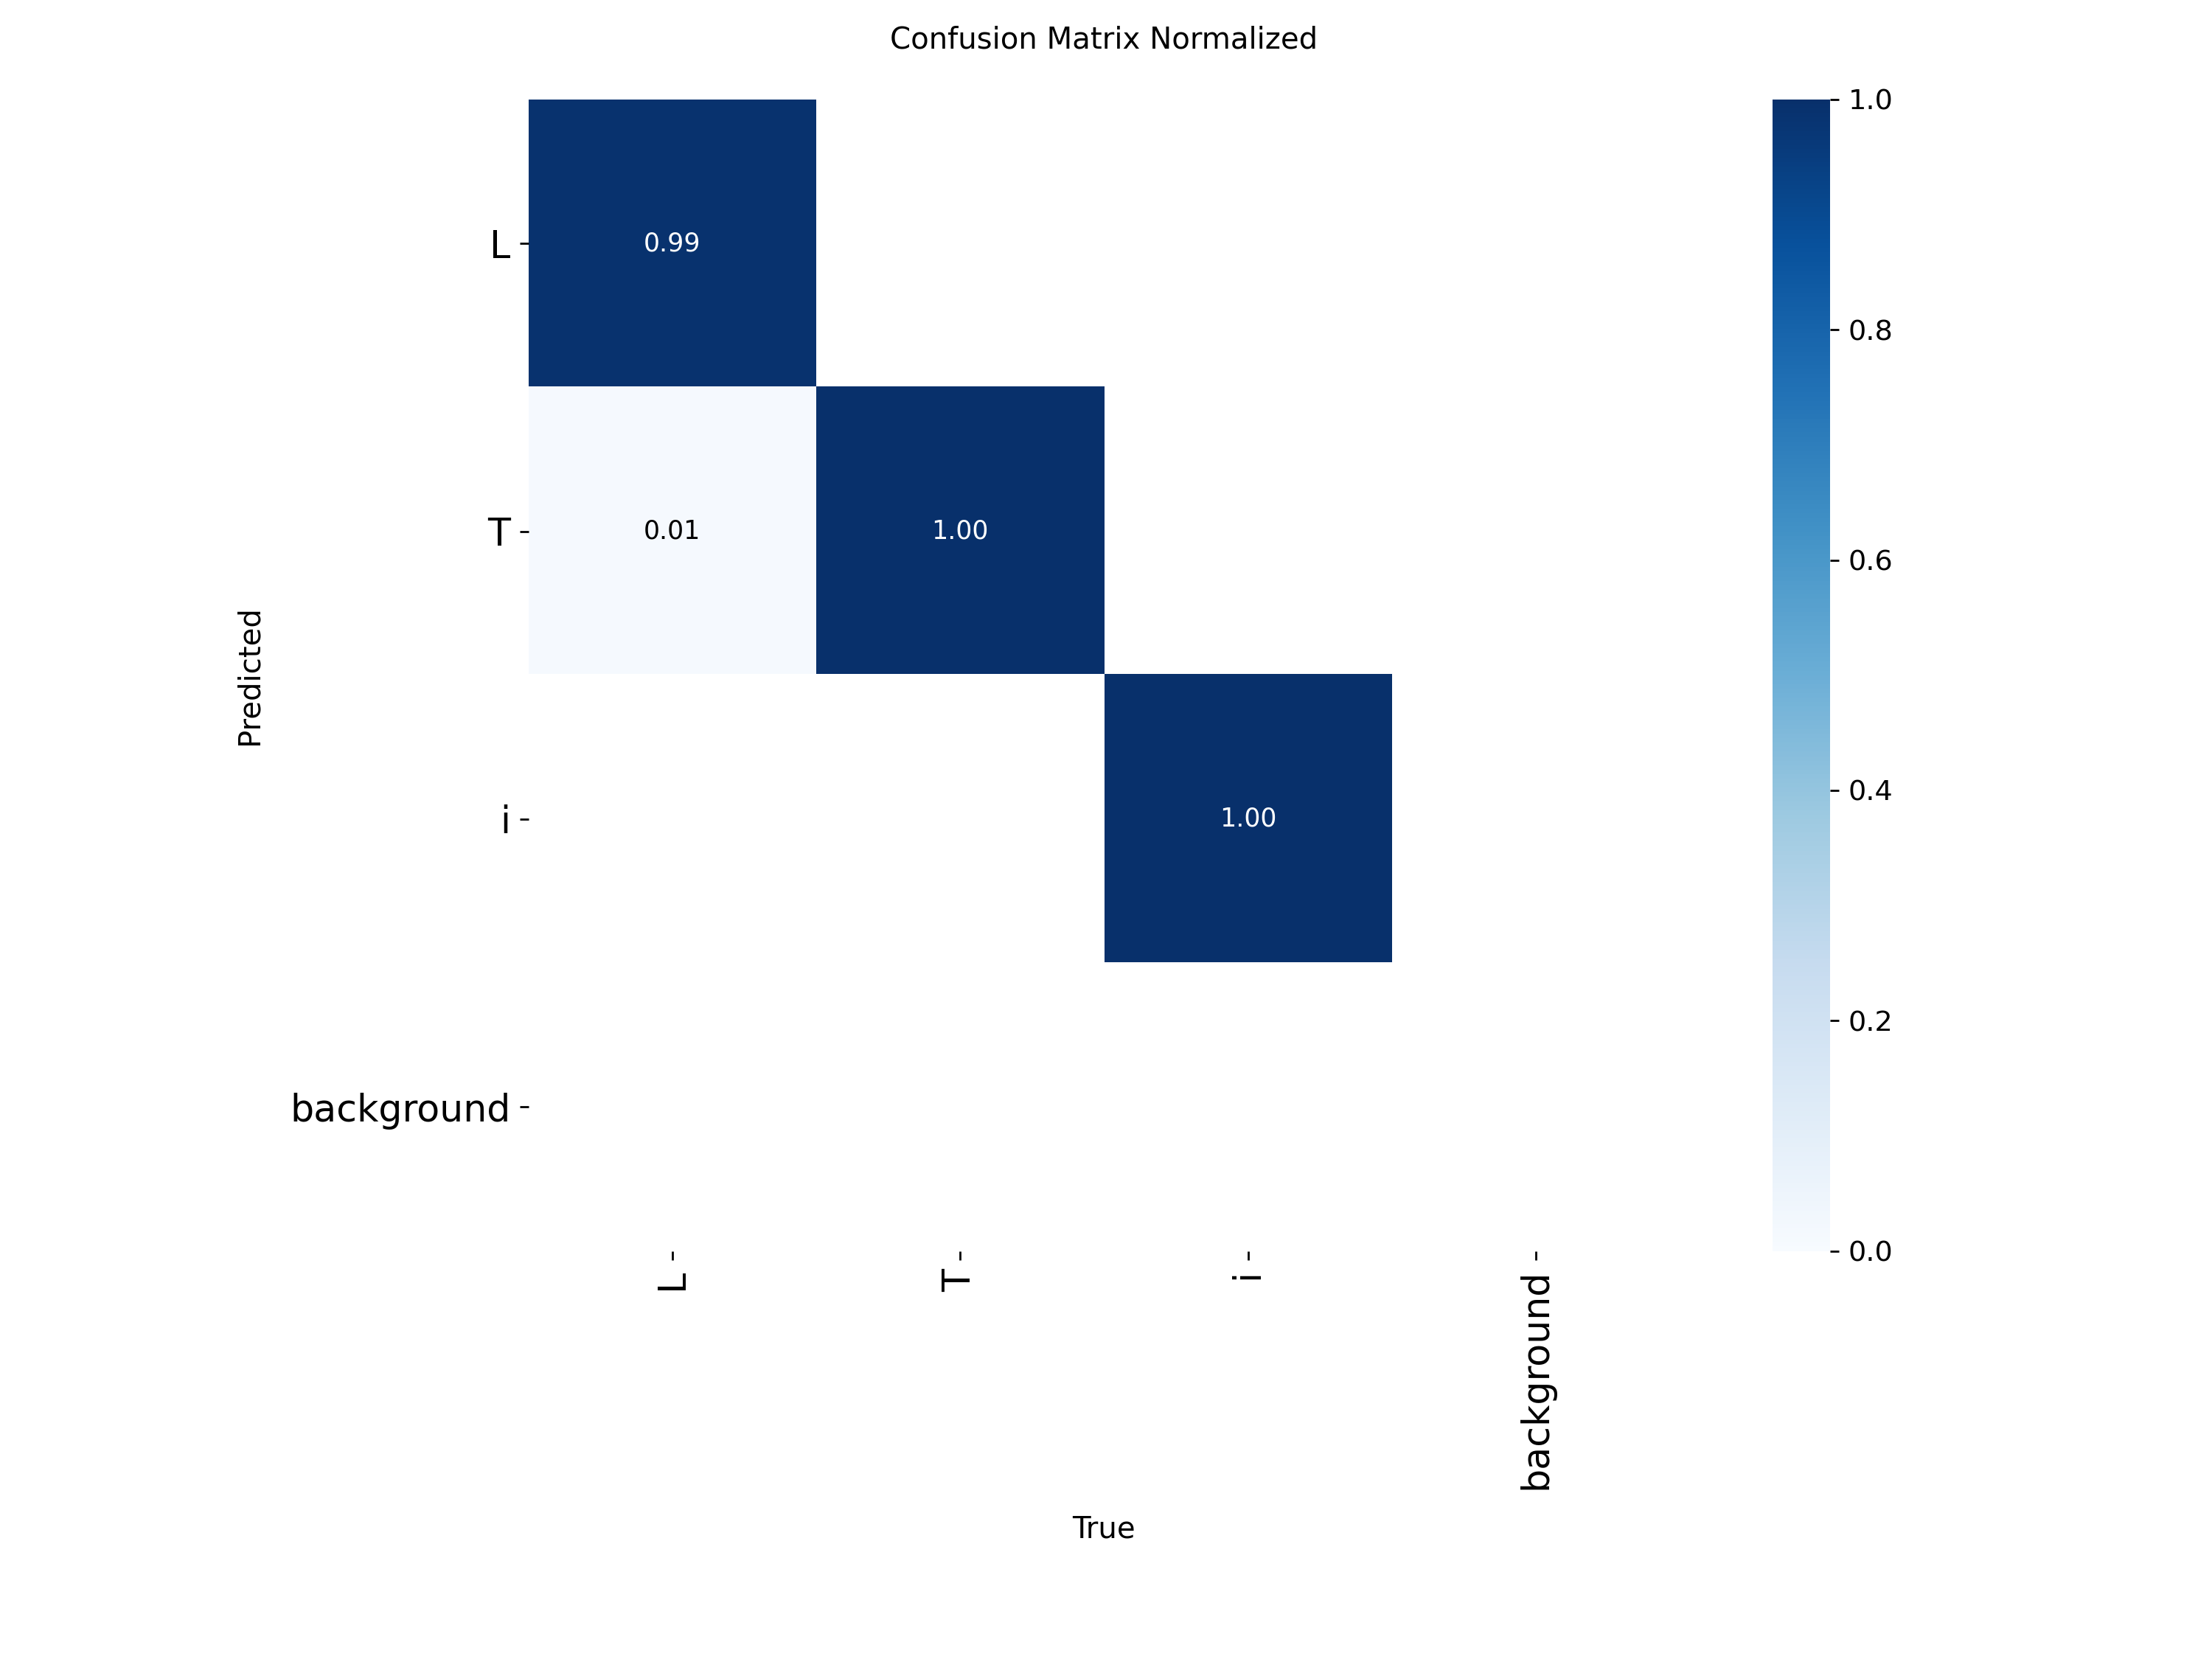
\includegraphics[width=0.7\textwidth]{Figures/chapter4/Detection/confusion_matrix_normalized.png}
    \caption{Normalized confusion matrix for brick classes.}
    \label{fig:det_confusion_matrix}
\end{figure}

\subsection{Precision--Recall Curves}
Precision--Recall (PR) curves summarize the tradeoff between precision and recall over varying confidence thresholds. We report separate PR curves for bounding boxes and segmentation masks.

\begin{figure}[H]
    \centering
    \begin{subfigure}[t]{0.48\textwidth}
        \centering
        \vspace{0pt}
        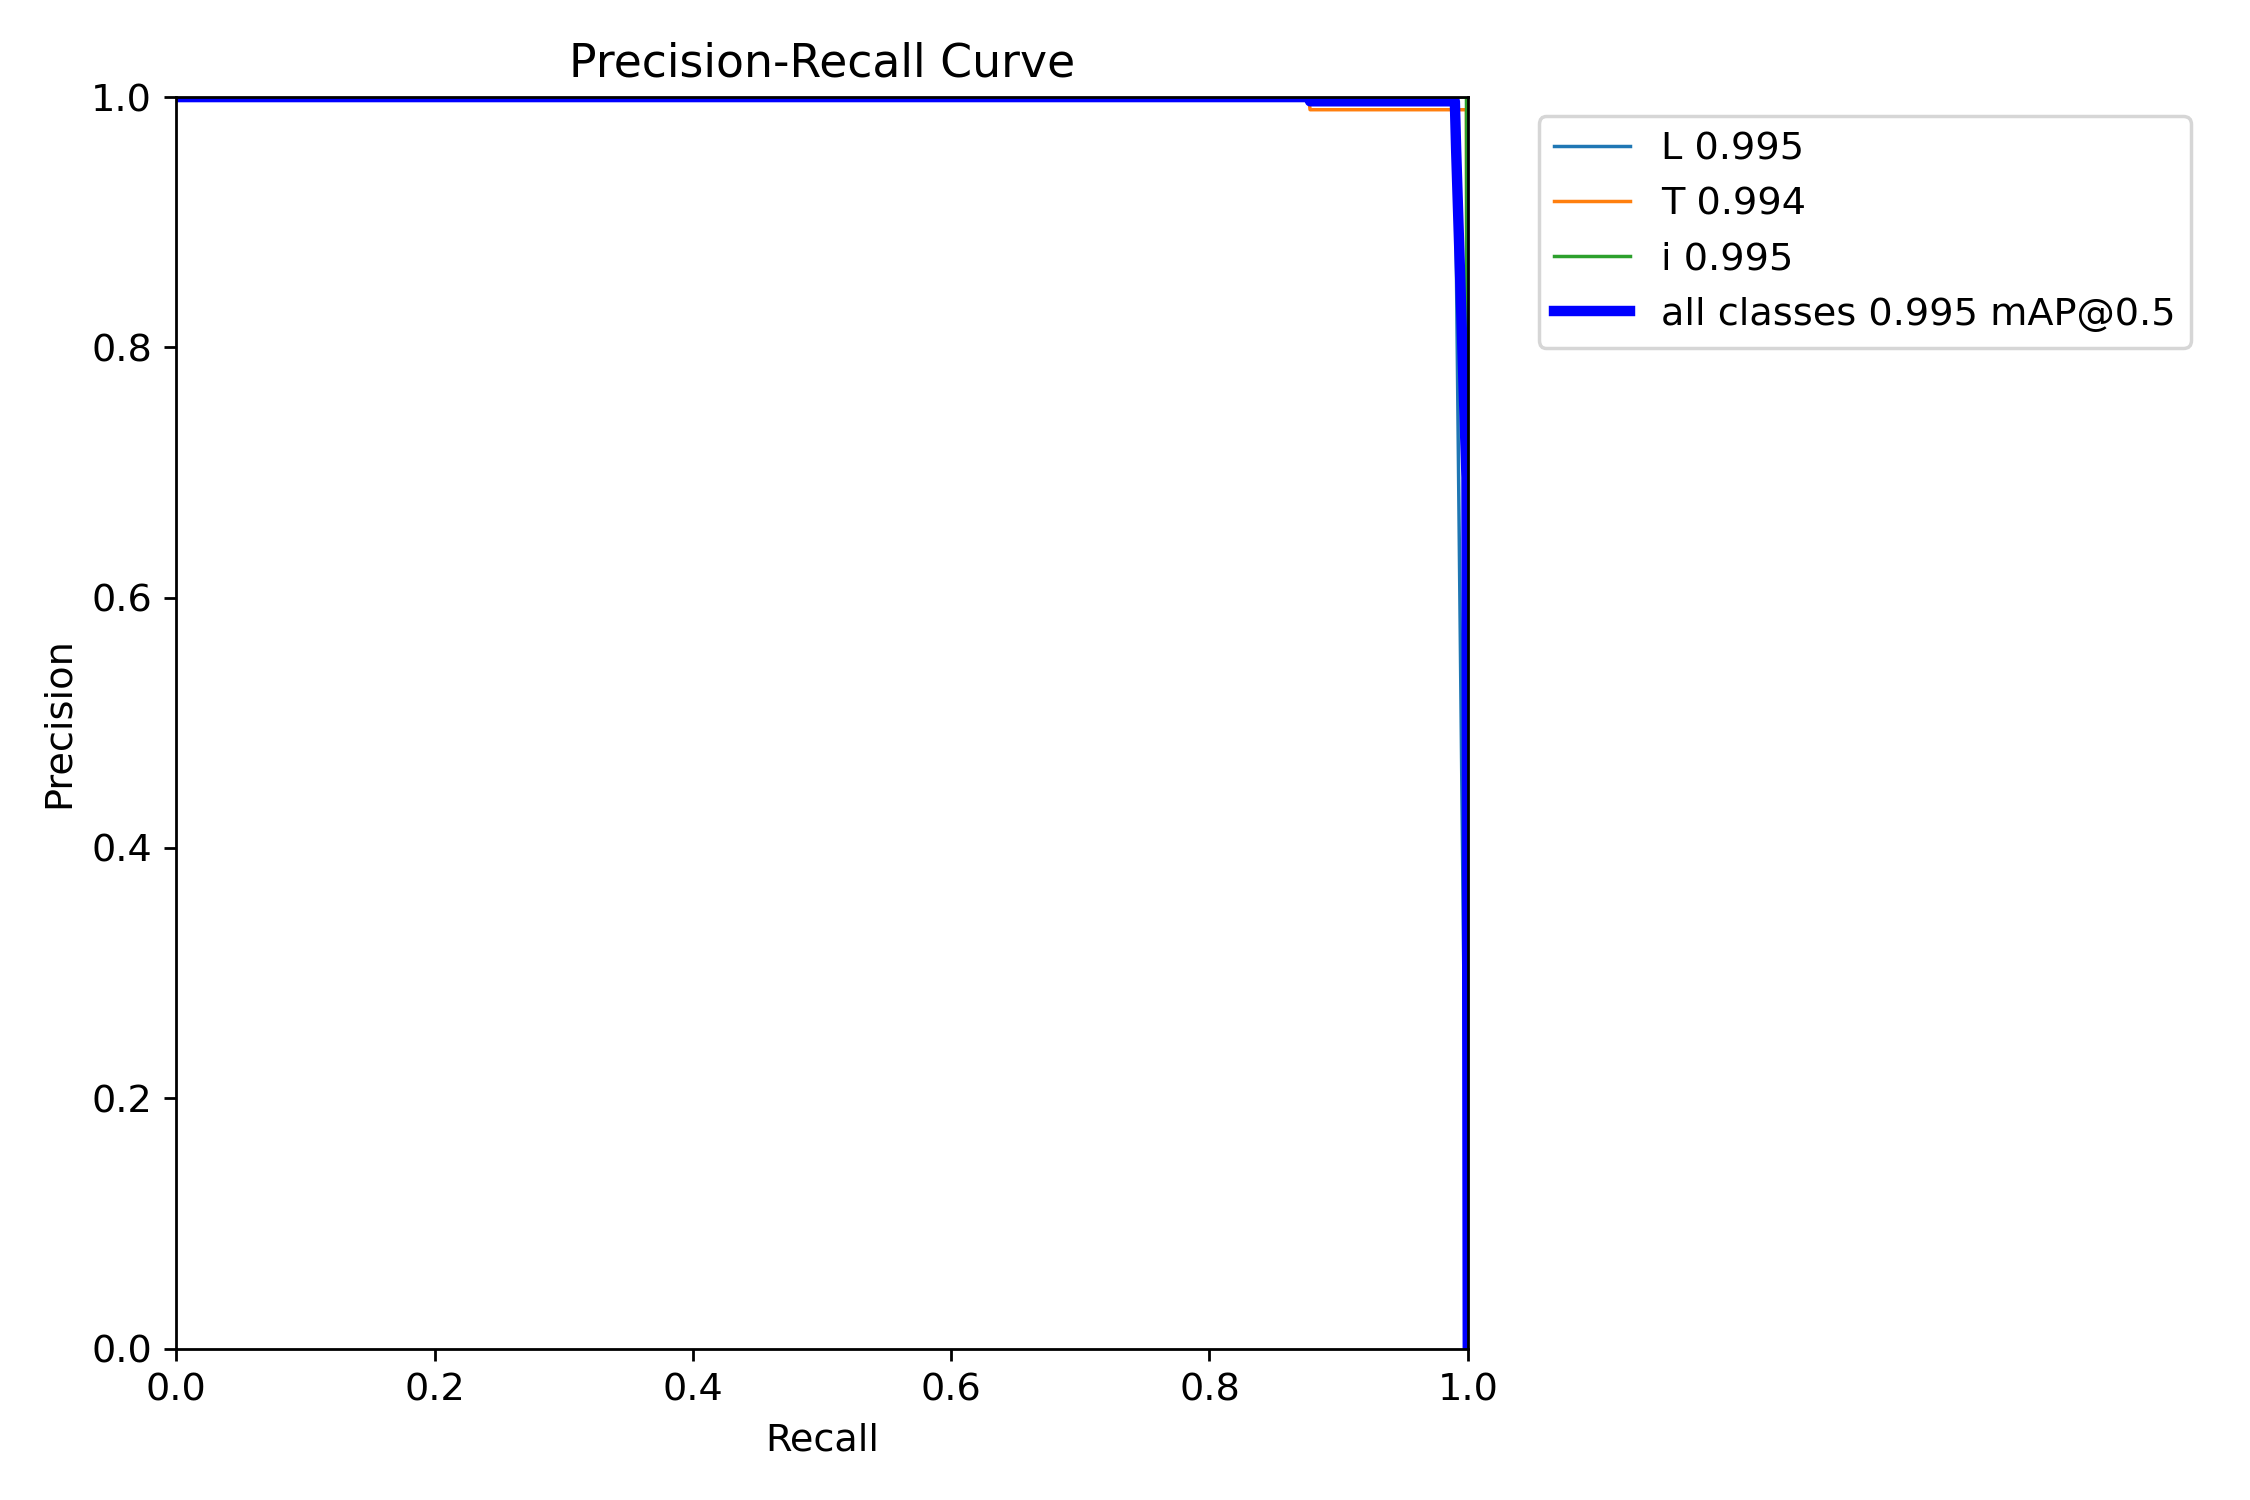
\includegraphics[width=\textwidth]{Figures/chapter4/Detection/BoxPR_curve.png}
        \caption{Box PR curve.}
        \label{fig:box_pr_curve}
    \end{subfigure}
    \begin{subfigure}[t]{0.48\textwidth}
        \centering
        \vspace{0pt}
        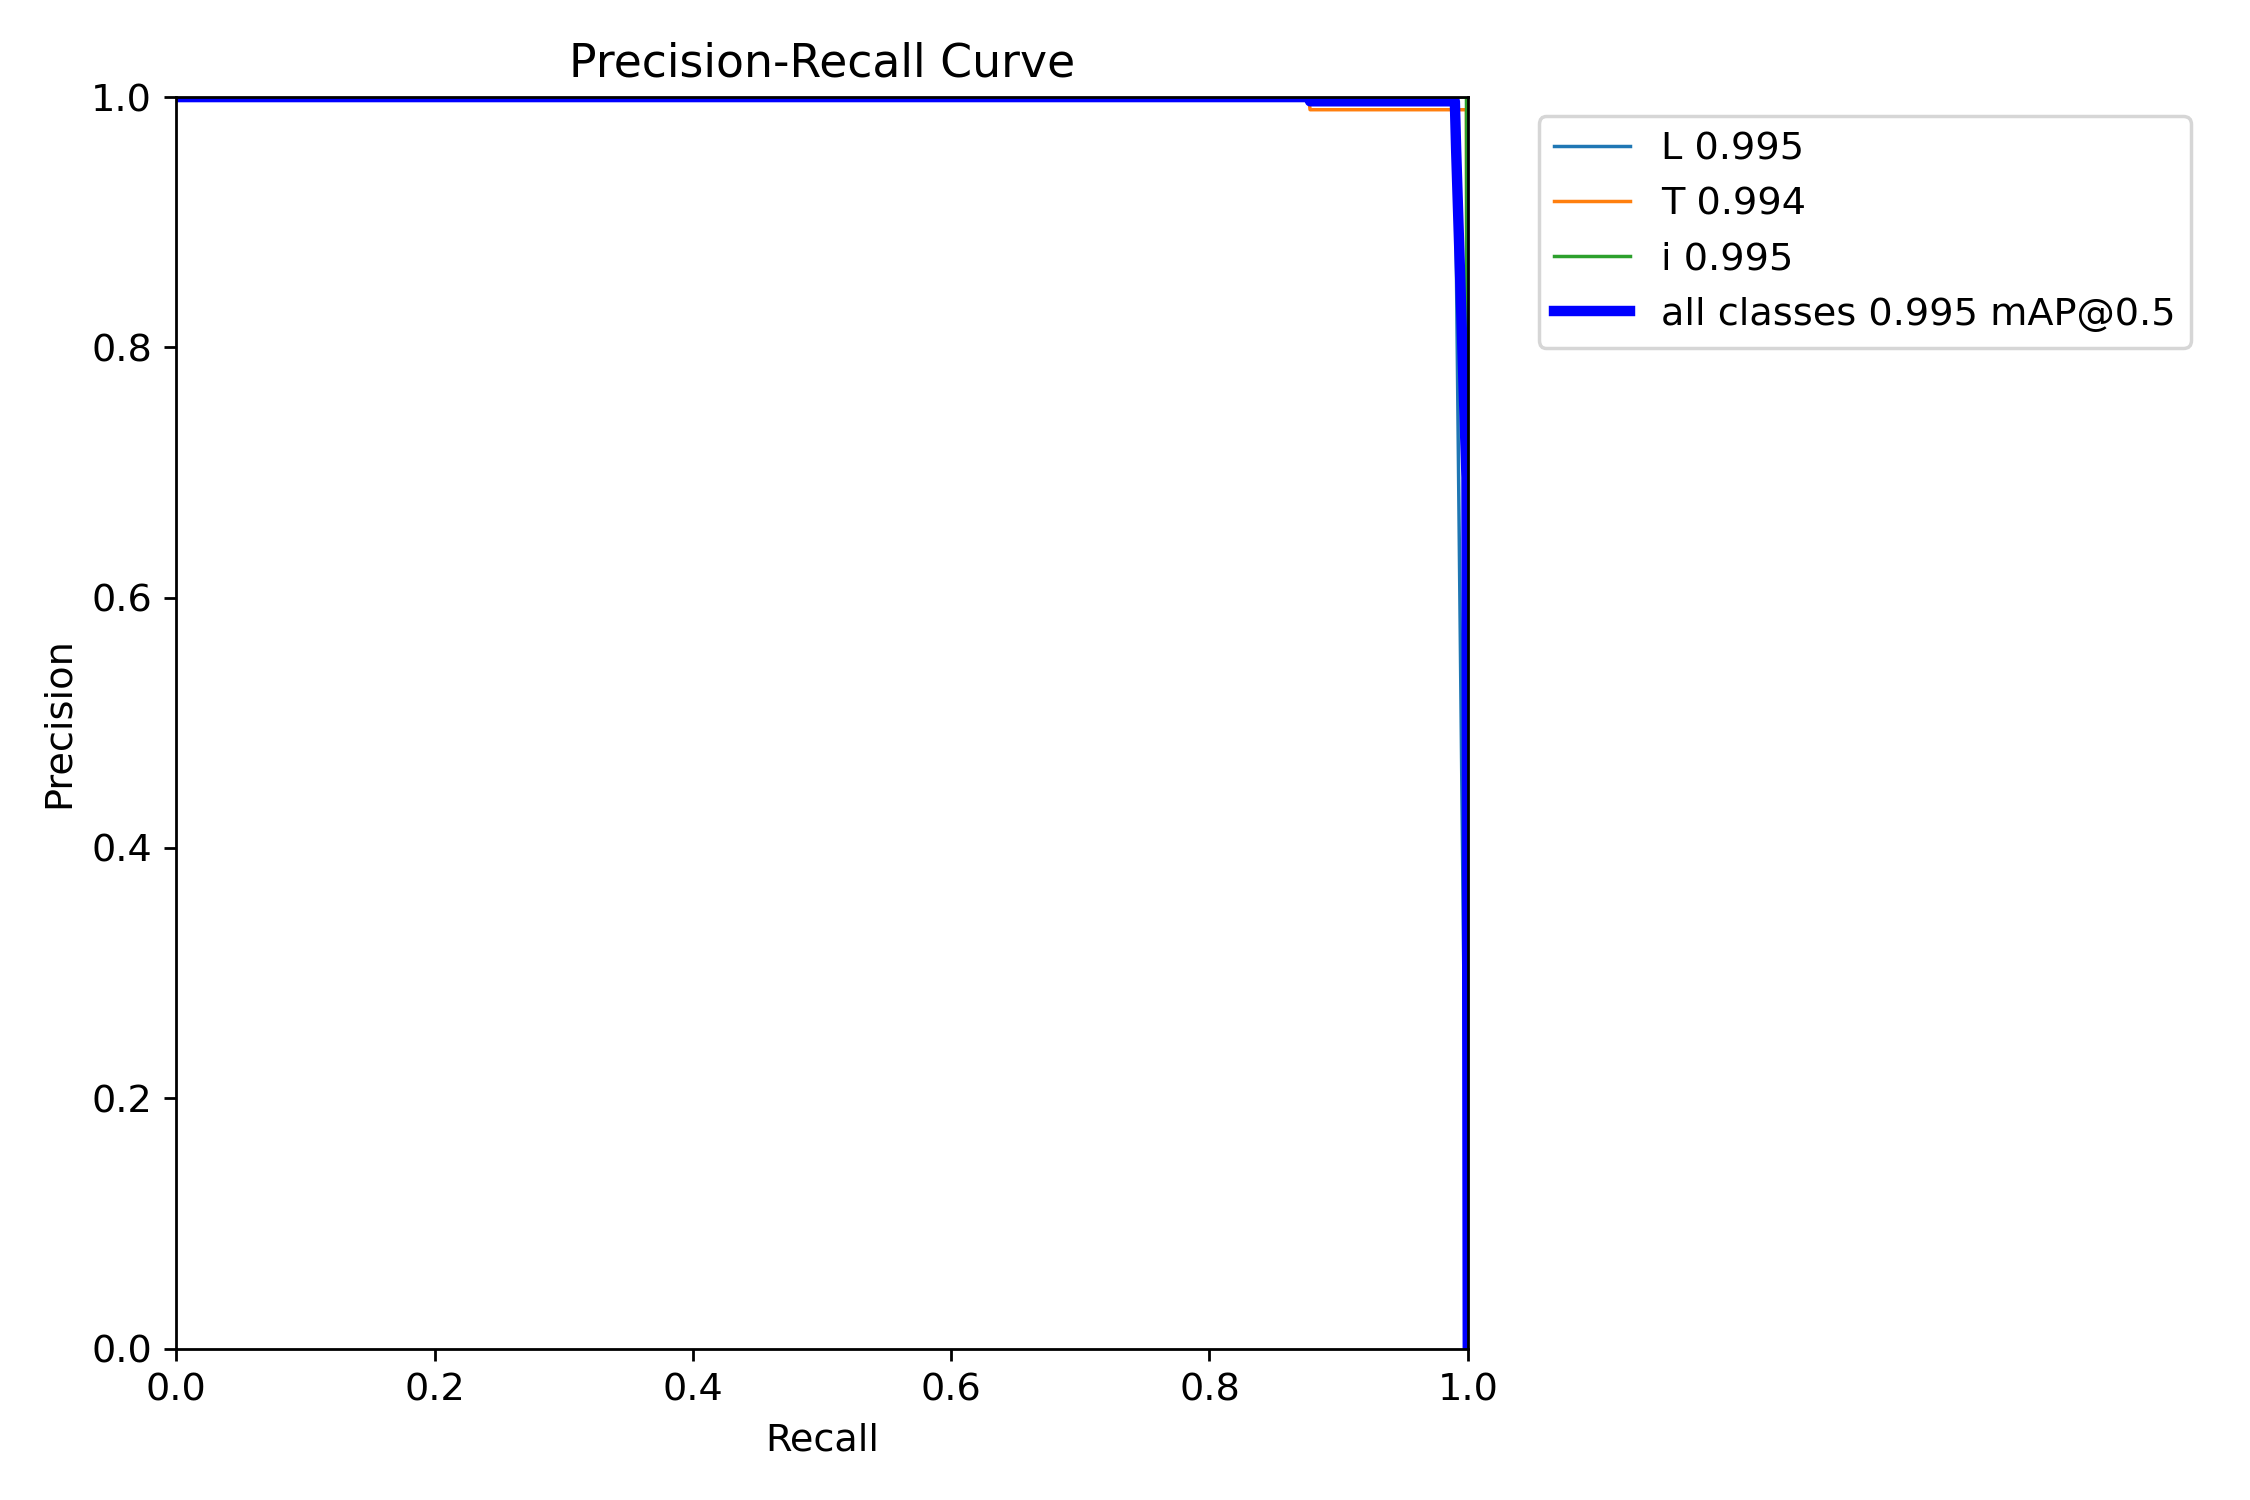
\includegraphics[width=\textwidth]{Figures/chapter4/Detection/MaskPR_curve.png}
        \caption{Mask PR curve.}
        \label{fig:mask_pr_curve}
    \end{subfigure}
    \caption{Precision--Recall curves for detection and segmentation.}
    \label{fig:det_pr_curves}
\end{figure}

\subsection{F1 Curves}
F1 curves indicate the balance between precision and recall across thresholds, which helps choose an operating point for deployment. We report F1 curves for both boxes and masks.

\begin{figure}[H]
    \centering
    \begin{subfigure}[t]{0.48\textwidth}
        \centering
        \vspace{0pt}
        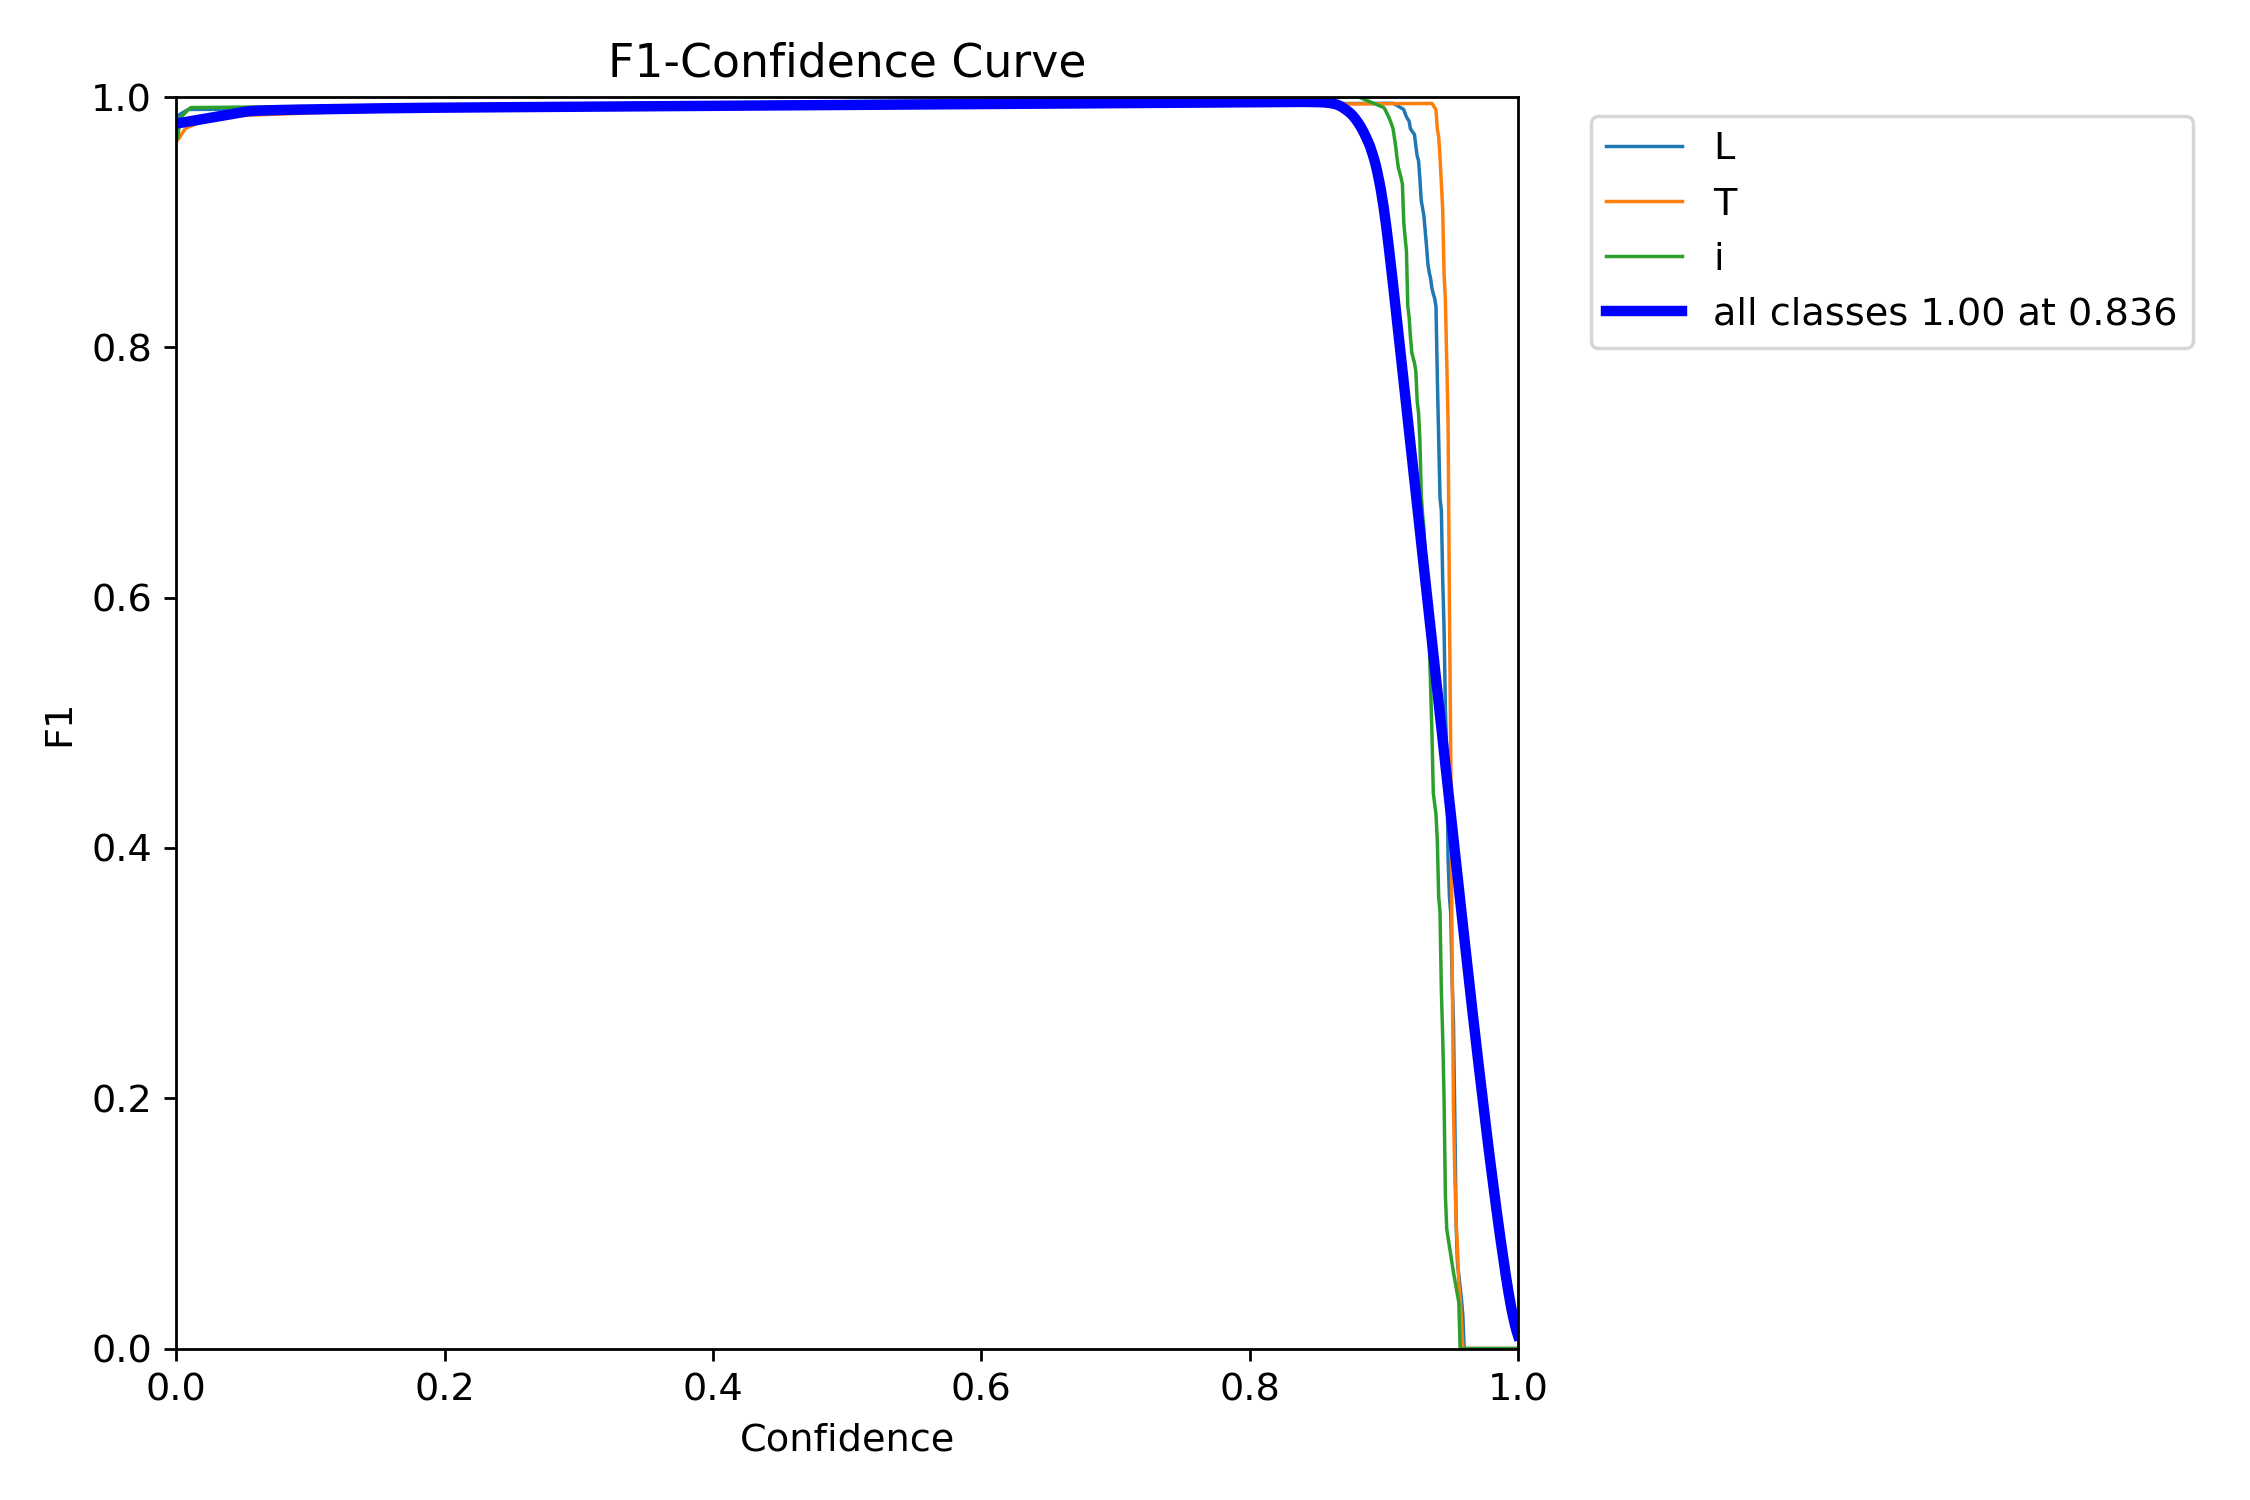
\includegraphics[width=\textwidth]{Figures/chapter4/Detection/BoxF1_curve.png}
        \caption{Box F1 curve.}
        \label{fig:box_f1_curve}
    \end{subfigure}
    \begin{subfigure}[t]{0.48\textwidth}
        \centering
        \vspace{0pt}
        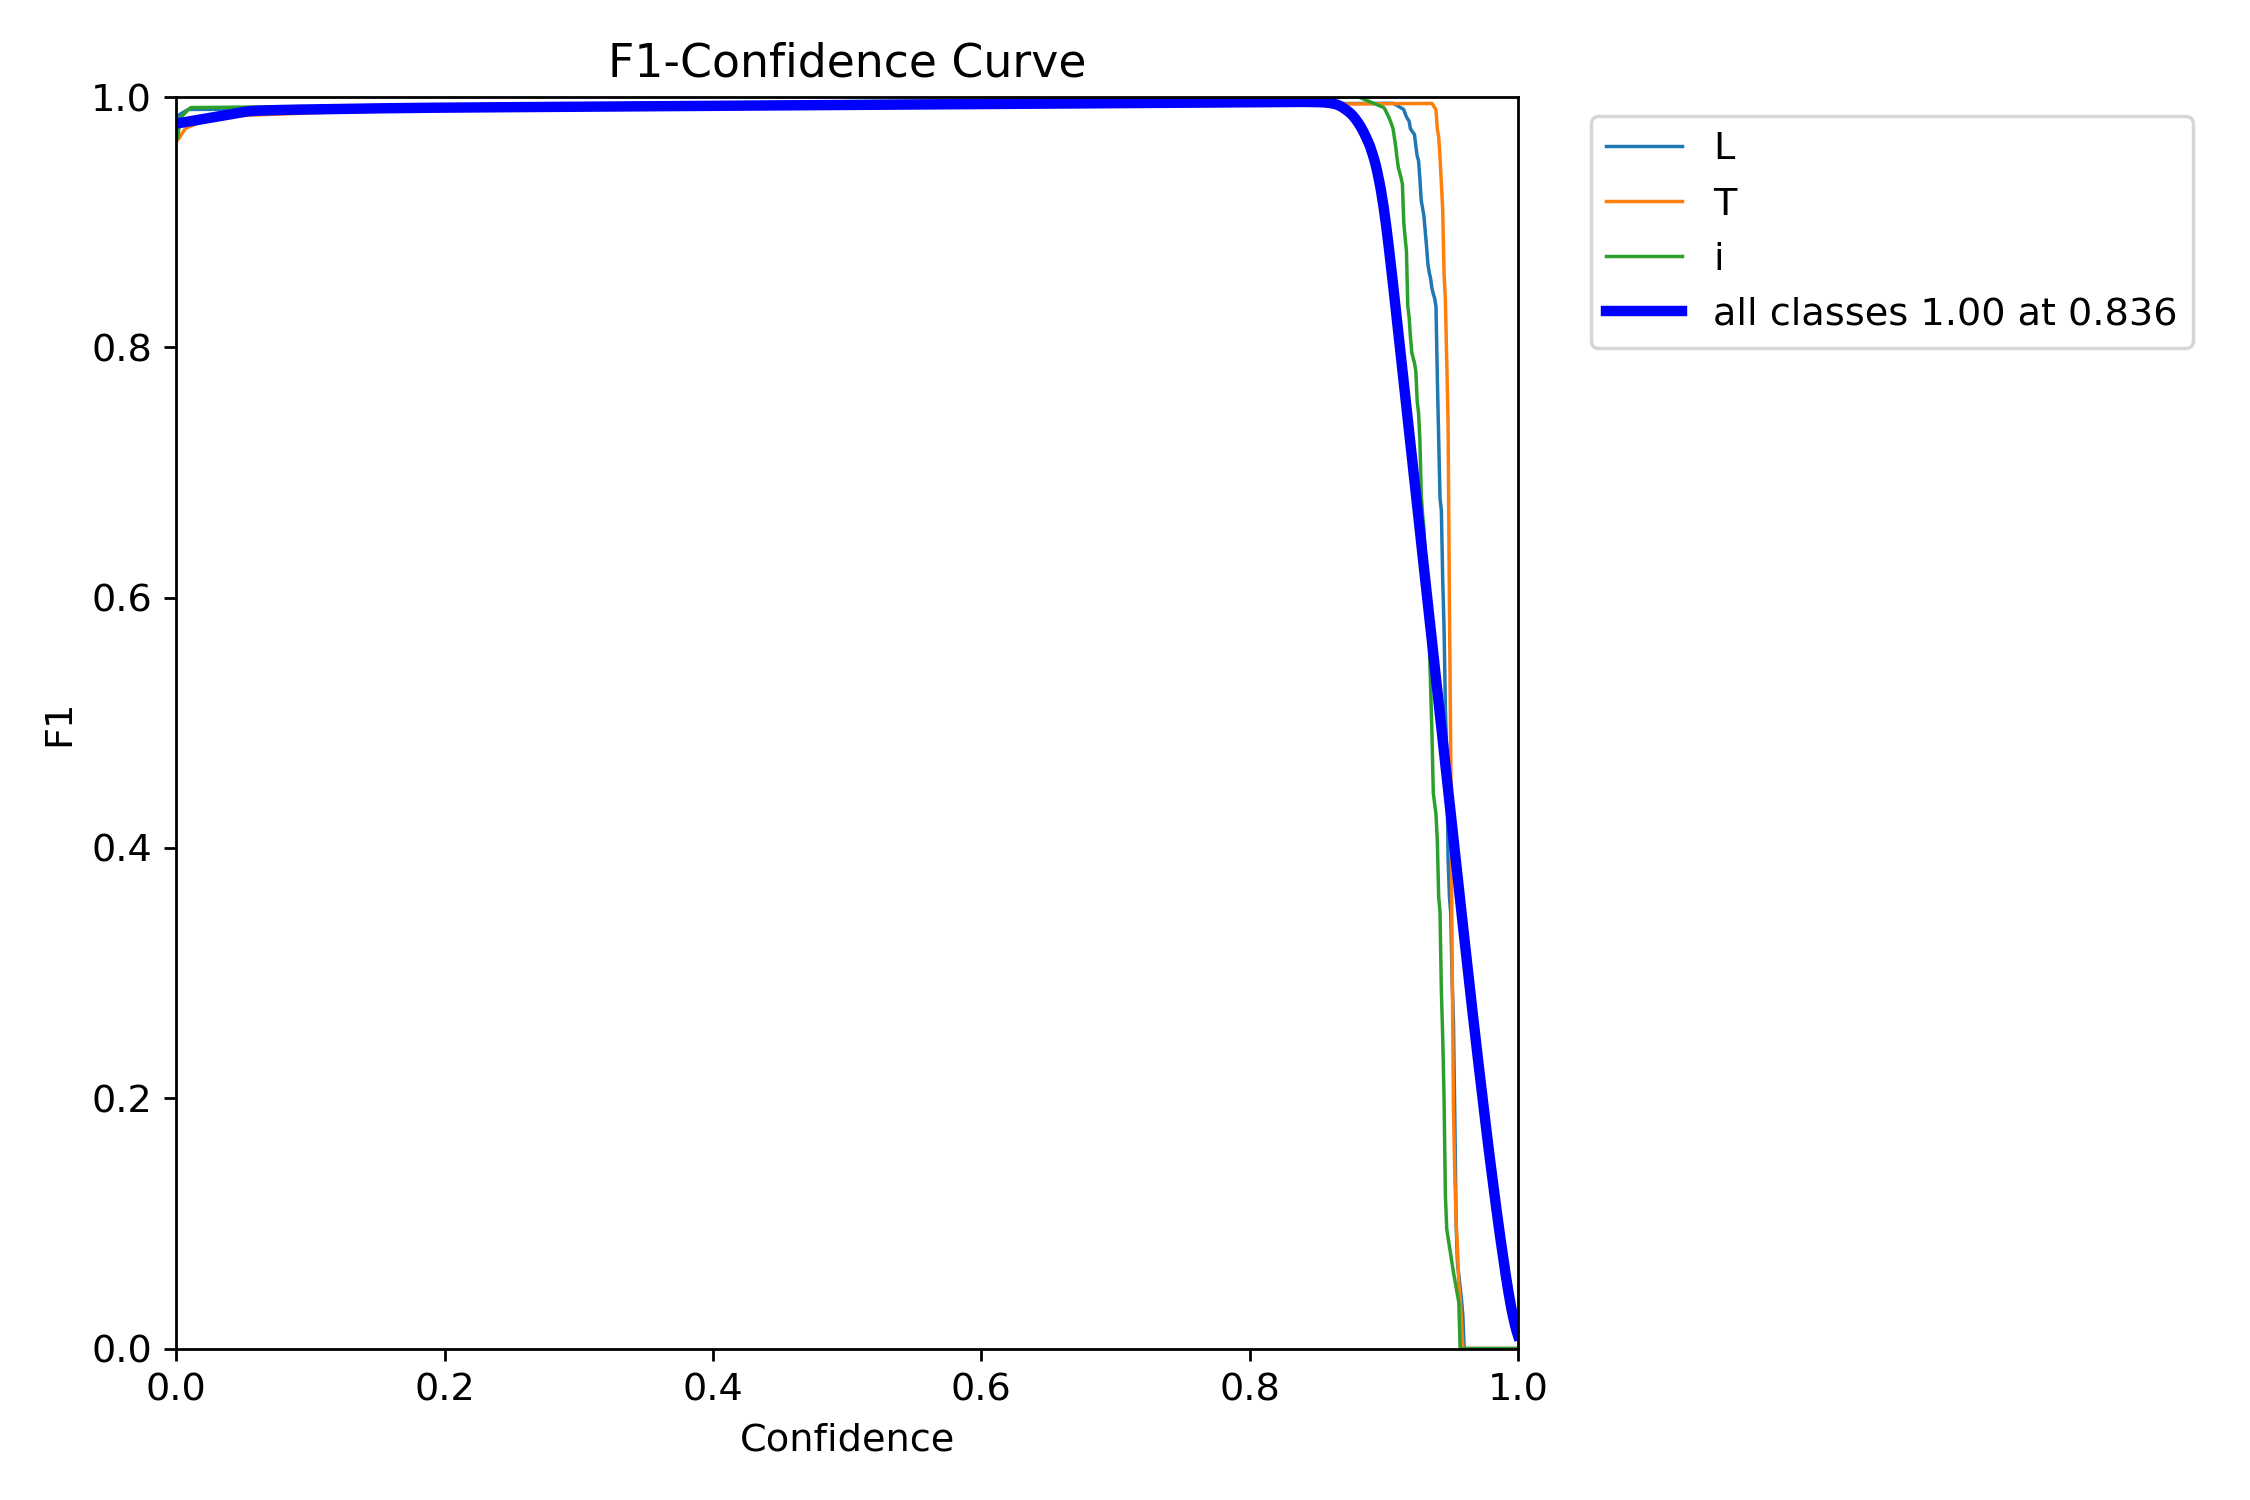
\includegraphics[width=\textwidth]{Figures/chapter4/Detection/MaskF1_curve.png}
        \caption{Mask F1 curve.}
        \label{fig:mask_f1_curve}
    \end{subfigure}
    \caption{F1 curves for detection and segmentation.}
    \label{fig:det_f1_curves}
\end{figure}

\subsection{Inference Results (Qualitative)}
To visualize the detection model in operation, Figure~\ref{fig:det_inference_examples} shows inference outputs on representative brick images. These examples highlight the predicted instances and their confidence for the three brick classes. The numeric labels shown next to each bounding box correspond to class IDs: \textbf{0 = L}, \textbf{1 = T}, and \textbf{2 = I}.

\begin{figure}[H]
    \centering
    \begin{subfigure}[t]{0.48\textwidth}
        \centering
        \vspace{0pt}
        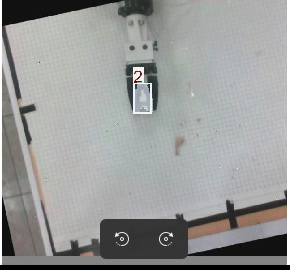
\includegraphics[width=\textwidth]{Figures/chapter4/Detection/inference/i.png}
        \caption{I-shape inference result.}
        \label{fig:det_infer_i}
    \end{subfigure}
    \begin{subfigure}[t]{0.48\textwidth}
        \centering
        \vspace{0pt}
        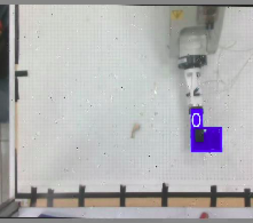
\includegraphics[width=\textwidth]{Figures/chapter4/Detection/inference/L.png}
        \caption{L-shape inference result.}
        \label{fig:det_infer_l}
    \end{subfigure}
    \vspace{0.4cm}
    \begin{subfigure}[t]{0.48\textwidth}
        \centering
        \vspace{0pt}
        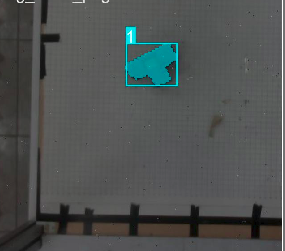
\includegraphics[width=\textwidth]{Figures/chapter4/Detection/inference/T.png}
        \caption{T-shape inference result.}
        \label{fig:det_infer_t}
    \end{subfigure}
    \begin{subfigure}[t]{0.48\textwidth}
        \centering
        \vspace{0pt}
        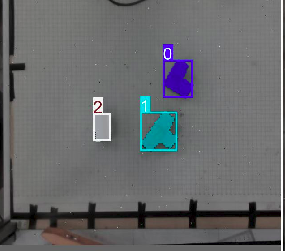
\includegraphics[width=\textwidth]{Figures/chapter4/Detection/inference/all.png}
        \caption{Mixed-scene inference result.}
        \label{fig:det_infer_all}
    \end{subfigure}
    \caption{Qualitative inference examples for YOLOv8s-seg detection.}
    \label{fig:det_inference_examples}
\end{figure}